% Created by tikzDevice version 0.12.3.1 on 2022-09-04 15:30:26
% !TEX encoding = UTF-8 Unicode
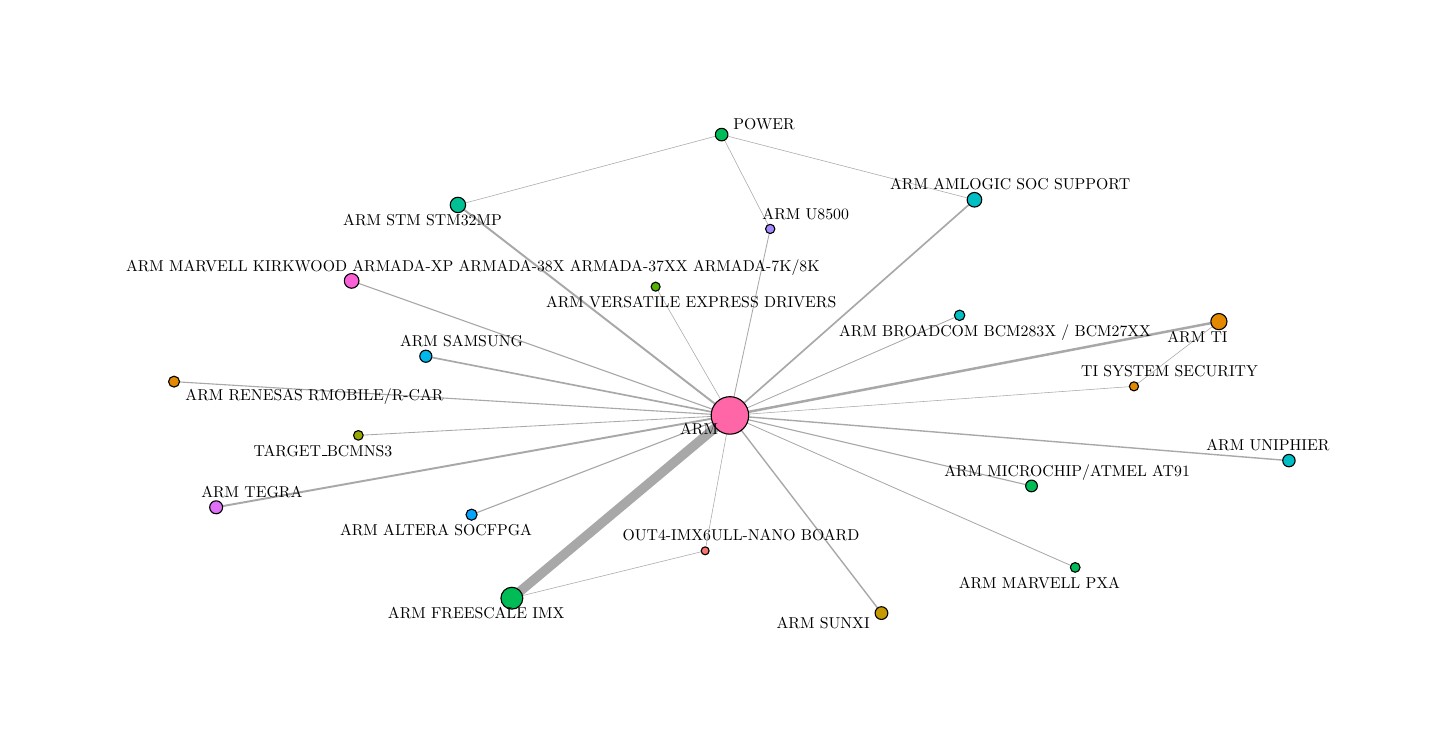
\begin{tikzpicture}[x=1pt,y=1pt]
\definecolor{fillColor}{RGB}{255,255,255}
\path[use as bounding box,fill=fillColor,fill opacity=0.00] (0,0) rectangle (505.89,252.94);
\begin{scope}
\path[clip] (  0.00,  0.00) rectangle (505.89,252.94);
\definecolor{fillColor}{RGB}{255,255,255}

\path[fill=fillColor] (  0.00,  0.00) rectangle (505.89,252.94);
\end{scope}
\begin{scope}
\path[clip] ( 32.75, 32.75) rectangle (475.89,222.94);
\definecolor{drawColor}{gray}{0.66}

\path[draw=drawColor,line width= 0.4pt,line join=round] (253.76,112.82) -- (160.40, 76.96);

\path[draw=drawColor,line width= 0.6pt,line join=round] (253.76,112.82) -- (342.12,190.75);

\path[draw=drawColor,line width= 0.3pt,line join=round] (253.76,112.82) -- (336.75,149.00);

\path[draw=drawColor,line width= 3.4pt,line join=round] (253.76,112.82) -- (174.96, 46.78);

\path[draw=drawColor,line width= 0.4pt,line join=round] (253.76,112.82) -- (117.06,161.44);

\path[draw=drawColor,line width= 0.3pt,line join=round] (253.76,112.82) -- (378.52, 57.90);

\path[draw=drawColor,line width= 0.4pt,line join=round] (253.76,112.82) -- (362.74, 87.34);

\path[draw=drawColor,line width= 0.4pt,line join=round] (253.76,112.82) -- ( 52.89,125.03);

\path[draw=drawColor,line width= 0.6pt,line join=round] (253.76,112.82) -- (143.87,134.21);

\path[draw=drawColor,line width= 0.7pt,line join=round] (253.76,112.82) -- (155.47,188.88);

\path[draw=drawColor,line width= 0.5pt,line join=round] (253.76,112.82) -- (308.51, 41.40);

\path[draw=drawColor,line width= 0.7pt,line join=round] (253.76,112.82) -- ( 68.10, 79.63);

\path[draw=drawColor,line width= 0.9pt,line join=round] (253.76,112.82) -- (430.45,146.73);

\path[draw=drawColor,line width= 0.3pt,line join=round] (253.76,112.82) -- (268.31,180.21);

\path[draw=drawColor,line width= 0.5pt,line join=round] (253.76,112.82) -- (455.75, 96.50);

\path[draw=drawColor,line width= 0.2pt,line join=round] (253.76,112.82) -- (226.91,159.34);

\path[draw=drawColor,line width= 0.2pt,line join=round] (253.76,112.82) -- (244.81, 63.90);

\path[draw=drawColor,line width= 0.3pt,line join=round] (253.76,112.82) -- (119.49,105.62);

\path[draw=drawColor,line width= 0.2pt,line join=round] (253.76,112.82) -- (399.76,123.33);

\path[draw=drawColor,line width= 0.2pt,line join=round] (342.12,190.75) -- (250.76,214.30);

\path[draw=drawColor,line width= 0.2pt,line join=round] (174.96, 46.78) -- (244.81, 63.90);

\path[draw=drawColor,line width= 0.2pt,line join=round] (155.47,188.88) -- (250.76,214.30);

\path[draw=drawColor,line width= 0.2pt,line join=round] (430.45,146.73) -- (399.76,123.33);

\path[draw=drawColor,line width= 0.2pt,line join=round] (268.31,180.21) -- (250.76,214.30);
\definecolor{drawColor}{RGB}{0,0,0}
\definecolor{fillColor}{RGB}{255,102,168}

\path[draw=drawColor,line width= 0.4pt,line join=round,line cap=round,fill=fillColor] (253.76,112.82) circle (  6.78);
\definecolor{fillColor}{RGB}{6,164,255}

\path[draw=drawColor,line width= 0.4pt,line join=round,line cap=round,fill=fillColor] (160.40, 76.96) circle (  2.01);
\definecolor{fillColor}{RGB}{0,191,196}

\path[draw=drawColor,line width= 0.4pt,line join=round,line cap=round,fill=fillColor] (342.12,190.75) circle (  2.64);

\path[draw=drawColor,line width= 0.4pt,line join=round,line cap=round,fill=fillColor] (336.75,149.00) circle (  1.88);
\definecolor{fillColor}{RGB}{0,188,86}

\path[draw=drawColor,line width= 0.4pt,line join=round,line cap=round,fill=fillColor] (174.96, 46.78) circle (  3.95);
\definecolor{fillColor}{RGB}{251,97,215}

\path[draw=drawColor,line width= 0.4pt,line join=round,line cap=round,fill=fillColor] (117.06,161.44) circle (  2.65);
\definecolor{fillColor}{RGB}{0,188,86}

\path[draw=drawColor,line width= 0.4pt,line join=round,line cap=round,fill=fillColor] (378.52, 57.90) circle (  1.75);

\path[draw=drawColor,line width= 0.4pt,line join=round,line cap=round,fill=fillColor] (362.74, 87.34) circle (  2.12);
\definecolor{fillColor}{RGB}{227,137,0}

\path[draw=drawColor,line width= 0.4pt,line join=round,line cap=round,fill=fillColor] ( 52.89,125.03) circle (  1.98);
\definecolor{fillColor}{RGB}{0,182,235}

\path[draw=drawColor,line width= 0.4pt,line join=round,line cap=round,fill=fillColor] (143.87,134.21) circle (  2.19);
\definecolor{fillColor}{RGB}{0,192,148}

\path[draw=drawColor,line width= 0.4pt,line join=round,line cap=round,fill=fillColor] (155.47,188.88) circle (  2.78);
\definecolor{fillColor}{RGB}{196,154,0}

\path[draw=drawColor,line width= 0.4pt,line join=round,line cap=round,fill=fillColor] (308.51, 41.40) circle (  2.30);
\definecolor{fillColor}{RGB}{223,112,248}

\path[draw=drawColor,line width= 0.4pt,line join=round,line cap=round,fill=fillColor] ( 68.10, 79.63) circle (  2.34);
\definecolor{fillColor}{RGB}{227,137,0}

\path[draw=drawColor,line width= 0.4pt,line join=round,line cap=round,fill=fillColor] (430.45,146.73) circle (  2.92);
\definecolor{fillColor}{RGB}{165,138,255}

\path[draw=drawColor,line width= 0.4pt,line join=round,line cap=round,fill=fillColor] (268.31,180.21) circle (  1.68);
\definecolor{fillColor}{RGB}{0,191,196}

\path[draw=drawColor,line width= 0.4pt,line join=round,line cap=round,fill=fillColor] (455.75, 96.50) circle (  2.24);
\definecolor{fillColor}{RGB}{83,180,0}

\path[draw=drawColor,line width= 0.4pt,line join=round,line cap=round,fill=fillColor] (226.91,159.34) circle (  1.63);
\definecolor{fillColor}{RGB}{248,118,109}

\path[draw=drawColor,line width= 0.4pt,line join=round,line cap=round,fill=fillColor] (244.81, 63.90) circle (  1.43);
\definecolor{fillColor}{RGB}{0,188,86}

\path[draw=drawColor,line width= 0.4pt,line join=round,line cap=round,fill=fillColor] (250.76,214.30) circle (  2.27);
\definecolor{fillColor}{RGB}{153,168,0}

\path[draw=drawColor,line width= 0.4pt,line join=round,line cap=round,fill=fillColor] (119.49,105.62) circle (  1.74);
\definecolor{fillColor}{RGB}{227,137,0}

\path[draw=drawColor,line width= 0.4pt,line join=round,line cap=round,fill=fillColor] (399.76,123.33) circle (  1.65);

\node[text=drawColor,anchor=base,inner sep=0pt, outer sep=0pt, scale=  0.57] at (242.62,106.05) {ARM};

\node[text=drawColor,anchor=base,inner sep=0pt, outer sep=0pt, scale=  0.57] at (147.56, 69.47) {ARM ALTERA SOCFPGA};

\node[text=drawColor,anchor=base,inner sep=0pt, outer sep=0pt, scale=  0.57] at (355.02,194.34) {ARM AMLOGIC SOC SUPPORT};

\node[text=drawColor,anchor=base,inner sep=0pt, outer sep=0pt, scale=  0.57] at (349.57,141.52) {ARM BROADCOM BCM283X / BCM27XX};

\node[text=drawColor,anchor=base,inner sep=0pt, outer sep=0pt, scale=  0.57] at (162.06, 39.29) {ARM FREESCALE IMX};

\node[text=drawColor,anchor=base,inner sep=0pt, outer sep=0pt, scale=  0.57] at (160.86,164.97) {ARM MARVELL KIRKWOOD ARMADA-XP ARMADA-38X ARMADA-37XX ARMADA-7K/8K};

\node[text=drawColor,anchor=base,inner sep=0pt, outer sep=0pt, scale=  0.57] at (365.58, 50.41) {ARM MARVELL PXA};

\node[text=drawColor,anchor=base,inner sep=0pt, outer sep=0pt, scale=  0.57] at (375.60, 90.89) {ARM MICROCHIP/ATMEL AT91};

\node[text=drawColor,anchor=base,inner sep=0pt, outer sep=0pt, scale=  0.57] at (103.65,118.20) {ARM RENESAS RMOBILE/R-CAR};

\node[text=drawColor,anchor=base,inner sep=0pt, outer sep=0pt, scale=  0.57] at (156.78,137.80) {ARM SAMSUNG};

\node[text=drawColor,anchor=base,inner sep=0pt, outer sep=0pt, scale=  0.57] at (142.67,181.42) {ARM STM STM32MP};

\node[text=drawColor,anchor=base,inner sep=0pt, outer sep=0pt, scale=  0.57] at (287.47, 35.77) {ARM SUNXI};

\node[text=drawColor,anchor=base,inner sep=0pt, outer sep=0pt, scale=  0.57] at ( 81.01, 83.19) {ARM TEGRA};

\node[text=drawColor,anchor=base,inner sep=0pt, outer sep=0pt, scale=  0.57] at (422.72,139.22) {ARM TI};

\node[text=drawColor,anchor=base,inner sep=0pt, outer sep=0pt, scale=  0.57] at (281.14,183.75) {ARM U8500};

\node[text=drawColor,anchor=base,inner sep=0pt, outer sep=0pt, scale=  0.57] at (448.17,100.07) {ARM UNIPHIER};

\node[text=drawColor,anchor=base,inner sep=0pt, outer sep=0pt, scale=  0.57] at (239.76,151.86) {ARM VERSATILE EXPRESS DRIVERS};

\node[text=drawColor,anchor=base,inner sep=0pt, outer sep=0pt, scale=  0.57] at (257.75, 67.50) {OUT4-IMX6ULL-NANO BOARD};

\node[text=drawColor,anchor=base,inner sep=0pt, outer sep=0pt, scale=  0.57] at (266.09,216.01) {POWER};

\node[text=drawColor,anchor=base,inner sep=0pt, outer sep=0pt, scale=  0.57] at (106.69, 98.15) {TARGET{\_{}}BCMNS3};

\node[text=drawColor,anchor=base,inner sep=0pt, outer sep=0pt, scale=  0.57] at (412.62,126.88) {TI SYSTEM SECURITY};
\end{scope}
\end{tikzpicture}
